\begin{definition}
    Функция дифференциируема в точке, если 
    \begin{itemize}
        \item $f:U \to \mathbb{R}^k$ и $p \in Int(U)$
        \item $f(x) = f(p) + df(p)\langle x-p \rangle + \alpha(x),$ где $\alpha(x) = o(x-p).$
    \end{itemize}
\end{definition}
Если $k = 1$, то лин. отображение $df(p):\mathbb{R}^n \to \mathbb{R}$
можно задатьа как $df(p)\langle v \rangle = \langle \nabla f(p);  v \rangle$
 - скалярное произведение градиента функции на вектор, причем 
 $\nabla f(p) = \left(\frac{\partial f}{\partial x_1}(p), \dots, \frac{\partial f}{\partial x_n}(p)\right)$ - вектор частных производных в точке $p$.

\begin{statement}
    Градиент функции задает направление, при движении в котором функция растет быстрее всего.
    \begin{proof}
        Рассмотрим функцию $f$ в точке $p$, вектор $v$ единичной длины будет задавать произвольное направление.
        \begin{equation*}\frac{f(p+tv) - f(p)}{t} \underset{t \to 0}{\to}
            \frac{\partial f}{\partial v} = df(p)\langle v \rangle = \langle \nabla f(p); v \rangle 
            = |\nabla f(p)| \cdot |v| \cdot cos(\varphi), \text{где $\varphi $ - угол между $\nabla f$ и $v$.}
        \end{equation*}
        Поскольку $|\nabla f(p) = const, |v| = 1$, то для максимизации надо выбрать такое $\varphi$, 
        чтобы $cos(varphi)$ был максимален, т.е. вектора $v$ и $\nabla f$ параллельны и $\nabla f$ задает наибольшую скорость роста.
    \end{proof}
\end{statement}

\begin{statement}
    $\nabla f(p)$ ортогонален поверхности уровня $\Omega = \{x | f(x) = c\}$.
    \begin{proof}
        Пусть $f(p) = c \ (p \in \Omega)$. Пусть $x_n \in \Omega$, покажем, что $cos(\nabla f(p), \overrightarrow{x_n-p}) \underset{n \to \infty}{\to} 0:$
        \begin{eqnarray*}
            f(x_n) = f(p) = c \implies 0 = f(x_n) - f(p) = df(p)\langle x_n-p \rangle + o(x_n - p) = 
            \langle \nabla f(p); x_n - p \rangle + o(x_n - p).
        \end{eqnarray*}
        Значит $0 \underset{n \to \infty}{=} \langle \nabla f(p); \frac{x_n - p}{|x_n - p|} \rangle + o(1)$, т.е.
        $\langle \nabla f(p); \frac{x_n - p}{|x_n - p|} \rangle \to 0 $. Тогда:
        \begin{equation*}
            \langle \nabla f(p); \frac{x_n - p}{|x_n - p|} \rangle = |\nabla f(p)|\cdot \left|\frac{x_n-p}{|x_n-p|}\right|\cdot cos(\alpha) \to 0, 
            \ \text{т.е.} \alpha \underset{n \to \infty}{\to} \frac{\pi}{2}. 
        \end{equation*}
        
    \end{proof}
\end{statement}

\begin{definition}
    Функция $f:\mathbb{R}^n \to \mathbb{R}^n$ называется векторным полем.
\end{definition}
\begin{definition}
    Потенциалом векторного поля $F$ (если он есть) называется \textbf{скалярная} функция $U:W \to \mathbb{R}$, 
    такая, что $\nabla U = F$. Если потенциал существует, то F называется потенциальным полем.

\end{definition}

\begin{theorem*}
    Пусть $f:U \subset \mathbb{R}^n \to \mathbb{R}^k, \ g:V \subset \mathbb{R}^k \to \mathbb{R}^m, \ f \in C^1(p), \ g \in C^1(q), \ q = f(p)$.\\
    Тогда $g \circ f \in C^1(p), \, dg \circ f = dg(f(p)) \cdot df(p).$ В матрицах Якоби: $D_{g \circ f}(p) = D_g(f(p)) \cdot D_f(p).$
\end{theorem*}

\begin{example}
    \begin{equation*}
        \begin{cases}
            f(x, y, z) = (xy, xz): \mathbb{R}^3 \to \mathbb{R}^2\\
            g(a, b) = \cosh(ab): \mathbb{R}^2 \to \mathbb{R}
        \end{cases} \quad
        f =
        \begin{cases}
            f_1(x, y, z) = xy\\
            f_2(x, y, z) = xz.
        \end{cases}
    \end{equation*}

    \begin{equation*}
        h = g(f(x, y, z)) = \cosh(xy \cdot xz): \mbox{R}^3 \to \mathbb{R}, \quad (x, y, z) \in \mathbb{R}^3 \overset{f}{\to} \mathbb{R}^3 \overset{g}{\to} \mathbb{R}
    \end{equation*}
    \begin{equation*}
        \frac{\partial h}{\partial x} = \sinh(x^2yz)\cdot 2xyz \quad
        \frac{\partial h}{\partial y} = \sinh(x^2yz)\cdot x^2z \quad
        \frac{\partial h}{\partial z} = \sinh(x^2yz) \cdot x^2y
    \end{equation*}

    \[D_f(x, y, z) = \begin{pmatrix}
        \frac{\partial f_1}{\partial x} & \frac{\partial f_1}{\partial y} &  \frac{\partial f_1}{\partial z} \\
        \frac{\partial f_2}{\partial x} & \frac{\partial f_2}{\partial y} &  \frac{\partial f_2}{\partial z}  
    \end{pmatrix} =
    \begin{pmatrix}
        y & x & 0 \\
        z & 0 & x
    \end{pmatrix}
    \]

    \[D_f = \begin{pmatrix}
        \sinh(ab)\cdot a & \sinh(ab) \cdot b
    \end{pmatrix}\]

    \[D_g \cdot D_f = \begin{pmatrix}
        \sinh(x^2yz)\cdot xz & \sinh(x^2yz)\cdot xy
    \end{pmatrix} \cdot \begin{pmatrix}
        y & x & 0 \\
        z & 0 & x
    \end{pmatrix}
    \]
    Досчитывать я это не буду, поверим Сторожуку на слово.
\end{example}

\textbf{Правило дифференциирования обратного отображения:}
Если невырождено и $\exists$ обратное отображение $g:V \to U$, непрерывное в точке $q = f(p)$, тогда:
\[g \in D(q) \text{ и } dg(q) = (df(p))^{-1}\]


\subsection{Многократная дифференциируемость}

\begin{definition}
    $f: U \subset \mathbb{R}^n \to \mathbb{R}^m \ k$ раз дифференциируема в точке $p$ ($f \in D^k(p)$), если:
    \begin{enumerate}
        \item $f$ дифференциируема во всех точках некоторой окрестности точки $p$;
        \item Все частные производные $\frac{\partial f}{\partial x_1}, \dots, \frac{\partial f}{\partial x_n}$ дифференциируемы $k-1$ раз в точке $p$.
    \end{enumerate}  
\end{definition}

\begin{example}
    \[f \in D^2(p) \implies f \in D(x) \text{ и } \frac{\partial f}{\partial x}, \frac{\partial f}{\partial y} \in D(p)  \]
\end{example}

\begin{statement*}
    Если $\begin{cases}
        f \in D^k(p): \mathbb{R}^n \to \mathbb{R}^k\\
        g \in D^k(p): \mathbb{R}^n \to \mathbb{R}^k
    \end{cases}$ тогда $h(x) = f(x) \cdot g(x) \in D^k(p)$

    \begin{proof}
        \begin{equation*}
            \frac{\partial h}{\partial x_i}(x) = \frac{\partial f}{\partial x_i}(x)\cdot g(x) +
            f(x) \cdot \frac{\partial g}{\partial x_i}
        \end{equation*}
        Так как $\frac{\partial f}{\partial x_i}(x) \in D^{k-1}(p), \ g(x) \in D^k(p), \ f(x) \in D^k(p), \ \frac{\partial g}{\partial x_i} \in D^{k-1}(p)$,
        то $\frac{\partial h}{\partial x_i} \in D^{k-1}(p)$.
    \end{proof}
\end{statement*}


\begin{theorem}[о вторых производных]
    Пусть $f:U \subset \mathbb{R}^n \to \mathbb{R}, \ f \in D^2(p)$. Тогда $\frac{\partial^2 f}{\partial x \partial y} = \frac{\partial^2 g}{\partial y \partial x}$.
    \begin{proof}
        Можно считать, что $n = 2$, так как при заданной функции $f(x_1, x_2, \dots)$ можно в качестве $f$ рассмотреть 
        сужение $f$ на плоскость $Ox_1x_2$, т.к. при дифференциировании по $x_1$ или $x_2$ остальные переменные не изменются.

        \[f = f(x, y) \in D^2(p), \quad p = (x_0, y_0, \dots)\]
        Считаем, что $p = 0$ и что $\frac{\partial f}{\partial x}(0) = 0, \ \frac{\partial f}{\partial y}(0) = 0$.
        Чтобы показать почему так можно считать введем $f_1$:
        \[f_1(x, y) := f(x,y) - f'_x(0, 0)\cdot x - f'_y(0,0)\cdot y\]
        \[\frac{\partial f_1}{\partial x}(0, 0) = \frac{\partial f}{\partial x}(0, 0) - f'_x(0,0)\]
        \[\frac{\partial f_1}{\partial y}(0,0) = \frac{\partial f}{\partial y}(0,0) - f'_y(0,0)\]
        
        Дальше считаем, что $f = f_1$ и $f(0,0) = 0$. 
        \begin{equation*}
            \frac{\partial f}{\partial x }(x, y) =f(0,0) + a_{11}\cdot x + a_{12}\cdot y + \alpha_1(x, y), \ \text{где }
            \alpha_1(x, y) = o(x, y), \ (a_{11}, a_{12}) = df(0,0)\langle x, y \rangle
        \end{equation*}
        По условию $\frac{\partial f}{\partial x}, \frac{\partial f}{\partial y} \in D(0)$, поэтому 
        $a_{11} = f_{xx}(0), \ a_{12} = f_{xy}(0)$.
        \[\frac{\partial f}{\partial y}(x, y) = f(0,0) + a_{21}\cdot x + a_{22}\cdot y + \alpha_2(x, y), \ 
        a_{21} = f_{yx}(0), \ a_{22} = f_{yy}(0)\]

        \newpage
        \begin{minipage}[t]{0.45\textwidth}        
            \begin{tikzpicture}[remember picture, overlay]
                \node[anchor=north west, yshift=5pt, xshift=10pt] at (current page.north west) {
                    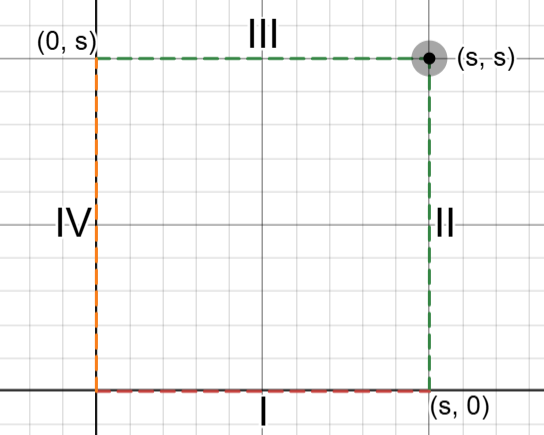
\includegraphics{График_для_теоремы_Шварца.png}
                };
            \end{tikzpicture}
        \end{minipage}
        \begin{minipage}[t]{0.5\textwidth}
            Рассмотрим точку $(s,s)$ вблизи нуля. Для нее 
            $f(s,s) - f(0,0) = (f(s,s) - f(s, 0)) + (f(s,0) - f(0,0)) = (II) + (I)$. \newline
            И в то же время $f(s, s) =  (\text{IV}) + (\text{III})$
        \end{minipage}
        \\[100pt]
        \[\text{II} = f(s,s) - f(s,0) = \int_{y=0}^{s}\frac{\partial f}{\partial y}(s,t)dt
        = \int_{t=0}^{s}a_{21}s + a_{22}t + \alpha_2(s,t)dt = a_{21}s^2 + \frac{a_{22}s^2}{2} + \varepsilon_1(s),\]
        причем $\varepsilon_1(s) = \int_{t=0}^{s}\alpha_2(s,t)dt$. Аналогично для I:
        \[\text{I} = f(s,0) - f(0,0) = \int_{t=0}^{s}\frac{\partial f}{\partial x}(t,0)dt = \int_{t=0}^{s}a_{11}t+a_{12}\cdot0 + \alpha_1(t)dt = 
        \frac{a_{11}}{2}s^2 + \varepsilon_2(s), \ \varepsilon_2(s) = \int_{t=0}^{s}\alpha_1(t,0)dt\]
        
        Итого: $f(s,s) - f(0,0) = \text{I} + \text{II} = s^2 \left( a_{21} + \frac{a_{11}}{2} + \frac{a_{22}}{2}+ \frac{\varepsilon_1(s) + \varepsilon_2(s)}{s^2}\right)$, что на самом деле равно $\text{III} + \text{IV} = 
        \\ = s^2\left(a_{12} + \frac{a_{11}}{2} + \frac{a_{22}}{2} + \frac{\varepsilon_3(s) + \varepsilon_4(s)}{s^2}\right)$
        
        \begin{equation}
            \label{eq}
            a_{21} + \frac{a_{11} + a_{22}}{2} + \frac{\varepsilon_1(s) + \varepsilon_2(s)}{s^2} = a_{12} + \frac{a_{22} + a{11}}{2} + \frac{\varepsilon_3(s) + \varepsilon_4(s)}{s^2}
        \end{equation}
        При малых $s$:
        \[\varepsilon_3(s) = \int_{t=0}^{s}\alpha_2(0, t)dt, \quad \varepsilon_3(s) = \int_{t=0}^{s}\alpha_1(t,s)dt\]
        Осталось показать, что $\varepsilon_{1,2,3,4} \underset{s \to 0}{=} o(s^2)$.
        Пусть $\varepsilon > 0$. Вспомним, что 
        \[\varepsilon_1(s) = \int_{t = 0}^{}\alpha_2(s,t)dt, \quad \alpha_2(x,y) \underset{x,y \to 0}{=} o(x,y)\]
        То есть, в некотором круге $V$ точки $(0,0)$ выполнено $\forall (x,y) \in V \quad \alpha_2(x,y) \leq \varepsilon \cdot \sqrt{x^2 + y^2}$.
        Для $s$ таких, что $(s,s) \in V \quad \alpha_2(x,y) \leq \varepsilon \cdot \sqrt{2} \cdot s$, при $\left| x \right| \leq s, \ \left| y \right| \leq s$.
        Тогда 
        \[\left| \varepsilon_1(s)\right| = \left| \int_{t=0}^{s}\alpha_2(s,t)dt \right| \leq \int_{t=0}^{s} \left|\alpha_2(s,t)\right|dt 
        \leq \int_{t=0}^{s}\varepsilon\cdot s\sqrt{2}\cdot dt = \varepsilon s^2\sqrt{2}\].
        Итак, мы доказали, что $\varepsilon_1(s) \underset{s \to 0}{=} o(s^2)$, аналогичным образом показываем для $\varepsilon_{2,3,4}$
        Тогда в равенстве \ref{eq} $\frac{\varepsilon_1(s) + \varepsilon_2(s)}{s^2} \to 0$ и $\frac{\varepsilon_3(s) + \varepsilon_4(s)}{s^2} \to 0$, а значит $a_{21} = a_{12}$,
        то есть $f_{xy}(0) = f_{yx}(0)$.
    \end{proof}
\end{theorem}

